% Customizable fields and text areas start with % >> below.
% Lines starting with the comment character (%) are normally removed before release outside the collaboration, but not those comments ending lines

% svn info. These are modified by svn at checkout time.
% The last version of these macros found before the maketitle will be the one on the front page,
% so only the main file is tracked.
% Do not edit by hand!
\RCS$Revision: 146736 $
\RCS$HeadURL: svn+ssh://emiglior@svn.cern.ch/reps/tdr2/notes/AN-12-308/trunk/AN-12-308.tex $
\RCS$Id: AN-12-308.tex 146736 2012-09-10 15:43:19Z emiglior $
%%%%%%%%%%%%% local definitions %%%%%%%%%%%%%%%%%%%%%
% This allows for switching between one column and two column (cms@external) layouts
% The widths should  be modified for your particular figures. You'll need additional copies if you have more than one standard figure size.
\newlength\cmsFigWidth
\ifthenelse{\boolean{cms@external}}{\setlength\cmsFigWidth{0.85\columnwidth}}{\setlength\cmsFigWidth{0.4\textwidth}}
\ifthenelse{\boolean{cms@external}}{\providecommand{\cmsLeft}{top}}{\providecommand{\cmsLeft}{left}}
\ifthenelse{\boolean{cms@external}}{\providecommand{\cmsRight}{bottom}}{\providecommand{\cmsRight}{right}}
%%%%%%%%%%%%%%%  Title page %%%%%%%%%%%%%%%%%%%%%%%%
\cmsNoteHeader{AN-13-XXX} % This is over-written in the CMS environment: useful as preprint no. for export versions
% >> Title: please make sure that the non-TeX equivalent is in PDFTitle below
\title{
Study of the muon momentum scale and resolution with MuScleFit on the $\sqrt{s}$ = 7 TeV and 8 TeV datasets}%
% >> Authors
%Author is always "The CMS Collaboration" for PAS and papers, so author, etc, below will be ignored in those cases
%For multiple affiliations, create an address entry for the combination
%To mark authors as primary, use the \author* form
\address[torino]{Universit\`a di Torino and INFN Sezione di Torino}
\author[torino]{S. Casasso, E. Migliore}

% >> Date
% The date is in yyyy/mm/dd format. Today has been
% redefined to match, but if the date needs to be fixed, please write it in this fashion.
% For papers and PAS, \today is taken as the date the head file (this one) was last modified according to svn: see the RCS Id string above.
% For the final version it is best to "touch" the head file to make sure it has the latest date.
\date{\today}

% >> Abstract
% Abstract processing:
% 1. **DO NOT use \include or \input** to include the abstract: our abstract extractor will not search through other files than this one.
% 2. **DO NOT use %**                  to comment out sections of the abstract: the extractor will still grab those lines (and they won't be comments any longer!).
% 3. **DO NOT use tex macros**         in the abstract: External TeX parsers used on the abstract don't understand them.
\abstract{
This note describes the studies on the momentum scale and on the resolution
of the muons reconstructed by the CMS experiment in the 2011 and 2012
proton-proton LHC runs using the MuScleFit algorithm.
Both real and simulated data were calibrated using the large sample
of dimuons decays from Z bosons. 
A data-driven validation of the results using dimuons from J/$\psi$,
$\Upsilon(1S)$ and Z decays and an estimate of the systematic
uncertainty on the momentum scale for the data collected in 2012 are
also presented. 
}

% >> PDF Metadata
% Do not comment out the following hypersetup lines (metadata). They will disappear in NODRAFT mode and are needed by CDS.
% Also: make sure that the values of the metadata items are sensible and are in plain text:
% (1) no TeX! -- for \sqrt{s} use sqrt(s) -- this will show with extra quote marks in the draft version but is okay).
% (2) no %.
% (3) No curly braces {}.
\hypersetup{%
pdfauthor={Stefano Casasso, Ernesto Migliore},%
pdftitle={
Study of the muon momentum scale and resolution with MuScleFit on the
\sqrt(s) = 7 TeV and 8 TeV datasets}, %
pdfsubject={CMS},%
pdfkeywords={CMS, physics, MUON}}

\maketitle %maketitle comes after all the front information has been supplied
% >> Text
%%%%%%%%%%%%%%%%%%%%%%%%%%%%%%%%  Begin text %%%%%%%%%%%%%%%%%%%%%%%%%%%%%
%% **DO NOT REMOVE THE BIBLIOGRAPHY** which is located before the appendix.
%% You can take the text between here and the bibiliography as an example which you should replace with the actual text of your document.
%% If you include other TeX files, be sure to use "\input{filename}" rather than "\input filename".
%% The latter works for you, but our parser looks for the braces and will break when uploading the document.
%%%%%%%%%%%%%%%
\renewcommand{\FIXME}{\noindent {\bf FIXME~}}
%%%%%%%%%%%%%%%%%%%%%%%%
\section{Introduction}
%%%%%%%%%%%%%%%%%%%%%%%%
\FIXME{Outline of Introduction}
\begin{itemize}
\item bla-bla on uncertainties in track reconstruction
\item definition of the datasets used
\item event/track selection
\item outline of the structure of the note
\end{itemize}
%The measurement of track momentum is affected by the reconstruction \ldots
%capability and our limited knowledge about the physical configuration
%of the detector. The main sources of biases in the momentum measurement are from residual misalignments and
%weak-modes, imprecisions in the magnetic field model, mismodelings of the material
%distribution/density. In this note the MuScleFit algorithm~\cite{XXX} is used to correct thise effects and extract an estimate %of the transverse momentum resolution. The method is based on an unbinned maximum
%likelihood fit to calibrate the data with a reference model of the J/y.
%This note is organized as follows: first a 

%%%%%%%%%%%%%%%%%%%%%%%%%%%%%
\section{Calibration strategy}
%%%%%%%%%%%%%%%%%%%%%%%%%%%%
The MuScleFit algorithm~\cite{CMS_AN_2010-059} uses the spectrum of dimuons from the decay of
reference resonances to determine biases in the momentum assigned to
charged tracks and to estimate its resolution.
For the calibration procedure described in this note, dimuons from the decay of
Z bosons were used. 
The invariant mass spectrum of the dimuons 
was modeled as the sum of a signal obtained from a NNLO
calculation~\cite{Dittmaier:2009cr}, adapted to kinematic cuts close to
those used in the selection of reconstructed muons, and an
exponentially falling background. The decay constants of the
exponential were determined separetely in nine bins depending on the
pseudorapidities of the two muons.
\FIXME add eta binning for the background model 
% $\eta(\mu^+)$ $\eta(\mu^-)$ 
%\FIXME description of MF strategy (scale no $p_0$, resolution, scale $p_0$ only, resolution) /ingredients\\
%\FIXME quote SDittmaier
%The ansatz functions describing the scale
%corrections and the resolution entering in the construction of
%the likelihood are detailed below.
%%%%%%%%%%%%%%%%%%%%%%%%%%%%%%%%%%%%%%%%%%%%%%%%%%%%%%
\subsection{Ansatz functions for scale corrections and resolution}
%%%%%%%%%%%%%%%%%%%%%%%%%%%%%%%%%%%%%%%%%%%%%%%%%%%%%%
%To derive a reference value of the mass of the 
%The reconstructed invariant mass specturm of the dimuon was fitted
%with the Table~\ref{tab:fit_pdfs}
Figure~\ref{fig:etaphi_44X_before} (left) shows the 
mass of the Z boson extracted from the reconstructed 
invariant mass spectrum of the dimuon in bins of
($\varphi$,$\eta$) of the positive muon for the data at
$\sqrt{s}$=7~TeV.
In each bin, the reconstructed invariant mass
was fitted with the pdf described in Table~\ref{tab:fit_pdfs}: 
the fitted pole of the Breit-Wigner was taken as the mass of the boson 
while the sigma of the Crystal Ball was taken as the resolution.
%%%%%%%
\begin{table}[hbH]
\begin{center}
\caption{Probability density functions (pdf's) used to extract the mass of
  the  J/$\psi$, $\Upsilon(1S)$ and Z resonances from the spectrum of
  the dimuon invariant mass $x$.
  $CB(x)$ is the Crystal Ball pdf, $BW(x)$ is the Breit-Wigner pdf,
  ``n$^{th}$ order Bern$(x)$'' is the n$^{th}$ order Bernstein
  polynomial pdf.\label{tab:fit_pdfs}}
\begin{tabular}{|ll|c|c|c|}
\hline
Resonance & & Fit Range [GeV] & Signal pdf & Background pdf \\
\hline
J/$\psi$       & DATA & [2.9,3.3] & $CB(x,\mu,\sigma)$ & 3$^{rd}$ order Bern. pol. \\
               & MC   & [2.9,3.3] & $CB(x,\mu,\sigma)$ & 3$^{rd}$ order Bern. pol. \\
\hline
$\Upsilon(1S)$ & DATA & [8.7,11.0] &$CB_(x,\mu_1,\sigma)+CB(x,\mu_2,\sigma)$ & 4$^{th}$ order Bern. pol. \\
               &      &            &$+CB(x,\mu_3,\sigma)$ & \\
               & MC   & [8.8,10.0] & $CB_(x,\mu,\sigma)$            & 4$^{th}$ order Bern. pol. \\
\hline
Z              & DATA & [75,105] & $BW(x,\mu,\Gamma_Z) \otimes CB(x,0,\sigma)$ & $\exp(a_0+a_1x+a_2x^2)$  \\
               & MC   & [75,105] & $BW(x,\mu,\Gamma_Z) \otimes CB(x,0,\sigma)$ & $\exp(a_0+a_1x+a_2x^2)$  \\
\hline
\end{tabular}
\end{center}
\end{table}
Offsets with respect the nominal mass of the Z up to 2 GeV are observed. 
Offsets are also observed in simulated events
(Figure~\ref{fig:etaphi_44X_before} right) as the conditions of 
the detector used in the reconstruction of simulated events reproduce the
level of knowledge of the detector in the data, hereafter referred to
as {\sl realistic} conditions.
\begin{figure}[hbtp]  
\begin{center}
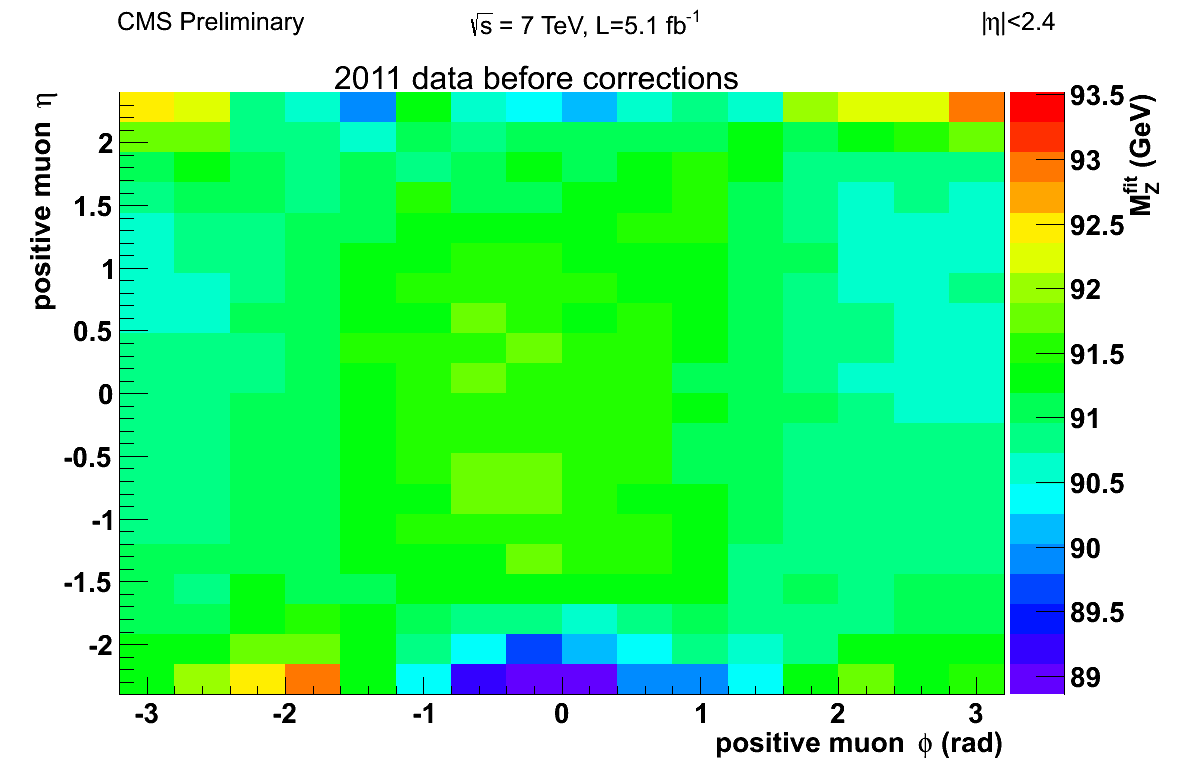
\includegraphics[width=0.45\textwidth]{figures/TkAl_Style/Data2011_44X/MassVsEtaPhiPlus_file0}
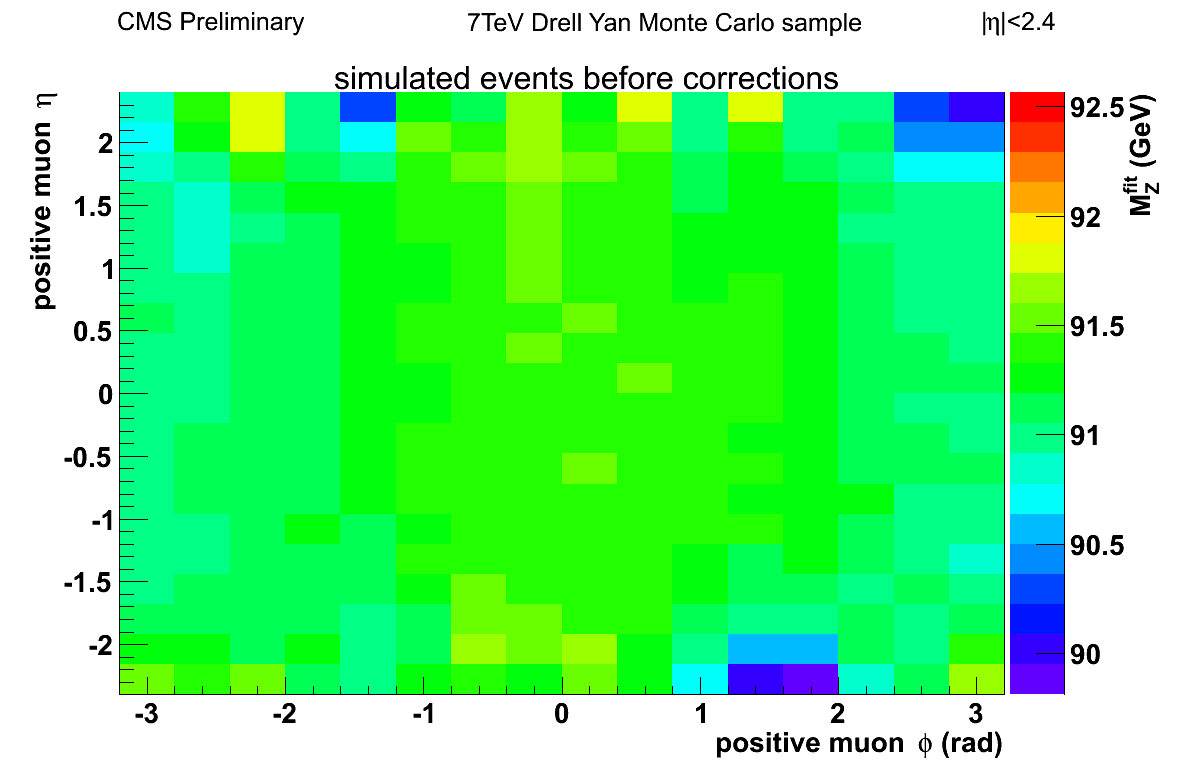
\includegraphics[width=0.45\textwidth]{figures/TkAl_Style/MC2011_44X/MassVsEtaPhiPlus_file0}
 \hspace{1cm} 
   \caption{Mass of the Z extracted from the specturm of the dimuon
     invariant mass for real (left) and simulated (right) events at $\sqrt{s}$=7 TeV, before
     applying the corrections computed with MuScleFit.
   \label{fig:etaphi_44X_before}}
 \end{center}
\end{figure} 
The bias in the assignment of the momentum is mainly
related to geometrical effects, e.g. deformations of the tracker
geometry used in the reconstruction still present after the
alignment procedure.
For this reason scale corrections were implemented as corrections to the curvature
$\kappa=q/p_T$ of the track. We modeled the corrections with an ansatz function defined in five
bins of the muon pseudorapidity: 
\begin{equation}
\kappa' = (1+p_0) \left( \kappa -\frac{\delta}{2} - C_j(\varphi,\eta)  \right),
\label{eq:scale_function}
\end{equation}
where $j$ is an index running on the $\eta$ bin: [-2.4,-2.1],
[-2.1,-1.5], [-1.5,+1.5], [+1.5,+2.1] and [+2.1,+2.4].\\
The terms in Eq.~\ref{eq:scale_function} are:
\begin{itemize}
\item $p_0$ corresponding to a global correction to the scale accounting for effects
  like inaccurate knowledge of the magnetic field;
\item $\delta$ representing an absolute bias in the curvature, e.g. a
  bias on the transverse momentum of the track different for negative
  and positive muons;
\item $C_j(\varphi,\eta)$ accounting for residual misalignment effects
  in each of the five $\eta$ bins.
  The functional form 
  \[
  C_j(\varphi,\eta) = a_{1,j} \sin(\varphi+\varphi_{1,j}) + a_{2,j}
  \sin(2\varphi+\varphi_{2,j}) + b_j(\eta-\eta_{0,j}) + b_{0,j} 
  \]
  was choosen to model the weak modes more frequently
  found in the post-alignment geometry, namely the sagitta (described
  by $a_{1,j}$), the
  twist (described by $b_j$) and the elliptical (described
  by $a_{2,j}$) deformations~\footnote{
    The three weak modes correspond to the following parametric deformations:
    $r\Delta\varphi = c_s \cos\varphi$ ``sagitta'',
    $\Delta\varphi = c_t z$  ``twist'' and 
    $\Delta r = r (1- c_e \cos 2\varphi)$  ``elliptical''
    with $c_s$, $c_t$ and $c_e$ being the approriate constants.}. 
  The elliptical deformations were considered null everywhere apart from 
  the first and last $\eta$ bin.
\end{itemize}
The resolution on $p_T$ was modeled as the sum in quadrature of two terms
\begin{equation}
\frac{\sigma(p_T)}{p_T}=q_0 p_T \oplus q_j ,
\label{eq:resolution_function}
\end{equation}
where the parameters $q_j$, representing multiple Coulomb scattering
effects, were computed separately in 12 equally spaced bins in $\eta$. 
\FIXME add a table/plot of the resolution parameters 
%%%%%%%%%%%%%%%%%%%%%%%%%%%%%%%%%%%%%%
\subsection{Fit strategy and results}
%%%%%%%%%%%%%%%%%%%%%%%%%%%%%%%%%%%%%%
The maximization of the likelihood was performed in four steps. First
values for the resolution function before any correction are
estimated. In the second step we fit all the parameters of the correction function with
the exception of the global scale $p_0$. Then 
the post-correction parameters of the resolution function are obtained.
The last step consists in fitting the global scale $p_0$. 
The fitted parameters were found to be stable against further
iterations of the maximization procedure.\\
Table~\ref{tab:scale_parameters} shows the values of the 
parameters of the correction function found by MuScleFit. 
Coefficients $a_{1,j}$, $a_{2,j}$ and $b_j$ with magnitude smaller than
0.000001 GeV$^{-1}$ were considered null. Similarly values
of $p_0$ smaller than 0.0050 were considered zero as they 
are consistent, within the systematic uncertainty 
computed in Section~\ref{sec:systematics}, with the null value.
%%%%%%%
\begin{sidewaystable}[hbH]
\begin{center}
\caption{Values of the fitted parameters for the scale
  correction~(Eq.~\ref{eq:scale_function}) for data and simulation
  samples at 7 TeV and 8 TeV. The five sections in the lower part
  of the table correspond to the five $\eta$ bins [-2.4,-2.1],
[-2.1,-1.5], [-1.5,+1.5], [+1.5,+2.1] and [+2.1,+2.4]. The values of
the $b_0$ parameters are fixed to guarantee the continuity of the
correction function at the boundaries between the $\eta$ bins.\label{tab:scale_parameters}} 
\begin{tabular}{|l|c|c|c|c|c|}
\hline
Sample & 2011\_DATA\_44X & 2011\_MC\_44X & 2012ABC\_DATA\_ReReco\_53X & 2012D\_DATA\_ReReco\_53X & 2012\_MC\_ReReco\_53X \\
\hline
$p_0$ & -0.00122  & 0.00000  & -0.00139  & -0.00135  & 0.00000  \\
\hline
$\delta$ & 0.00004  & 0.00004  & 0.00004  & 0.00004  & 0.00005  \\
\hline
$a_1$ & 0.00080  & 0.00022  & 0.00028  & 0.00025  & 0.00027  \\
$\phi_1$ & 1.33254  & 0.28482  & 1.21602  & 1.21894  & 0.14179  \\
$a_2$ & 0.00041  & 0.00030  & 0.00019  & 0.00017  & 0.00023  \\
$\phi_2$ & 1.79848  & -1.68476  & 1.78374  & 1.93410  & -1.71046  \\
$b$ & -0.00013  & -0.00007  & -0.00004  & -0.00005  & 0.00000  \\
%$\eta_0$ (fixed) & -2.10000  & -2.10000  & -2.10000  & -2.10000  & -2.10000  \\
$b_0$ & 0.00010  & -0.00001  & 0.00003  & 0.00004  & -0.00002  \\
\hline
$a_1$ & 0.00009  & 0.00006  & 0.00002  & 0.00000  & 0.00001  \\
$\phi_1$ & 1.17708  & -1.13170  & 0.26269  & 0.15297  & -1.04015  \\
$b$ & -0.00024  & 0.00003  & -0.00008  & -0.00009  & 0.00004  \\
%$\eta_0$ (fixed) & -1.50000  & -1.50000  & -1.50000  & -1.50000  & -1.50000  \\
$b_0$ & -0.00004  & 0.00000  & -0.00002  & -0.00002  & 0.00000  \\
\hline
$a_1$ & 0.00015  & 0.00007  & 0.00007  & 0.00007  & 0.00007  \\
$\phi_1$ & -1.30574  & -1.75023  & -1.24722  & -1.39464  & -1.64733  \\
$b$ & 0.00003  & 0.00000  & 0.00001  & 0.00001  & 0.00000  \\
\hline
$a_1$ & 0.00001  & 0.00013  & 0.00002  & 0.00001  & 0.00003  \\
$\phi_1$ & 0.89885  & -1.40495  & 0.21788  & 1.17093  & -1.68410  \\
$b$ & -0.00018  & 0.00000  & -0.00003  & -0.00003  & 0.00000  \\
%$\eta_0$ (fixed) & 1.50000  & 1.50000  & 1.50000  & 1.50000  & 1.50000  \\
$b_0$ & 0.00004  & 0.00000  & 0.00002  & 0.00002  & 0.00000  \\
\hline
$a_1$ & 0.00058  & 0.00014  & 0.00021  & 0.00032  & 0.00018  \\
$\phi_1$ & 1.85334  & -1.42615  & 1.94164  & 1.89407  & -0.94791  \\
$a_2$ & 0.00028  & 0.00001  & 0.00012  & 0.00008  & 0.00012  \\
$\phi_2$ & -0.84138  & 0.78290  & -1.10183  & -1.23759  & 0.38600  \\
$b$ & -0.00020  & -0.00001  & -0.00008  & -0.00010  & 0.00000  \\
%$\eta_0$ (fixed) & 2.10000  & 2.10000  & 2.10000  & 2.10000  & 2.10000  \\
$b_0$ & -0.00006  & 0.00000  & -0.00001  & 0.00000  & 0.00000  \\
\hline
\hline
\end{tabular}
\end{center}
\end{sidewaystable}

Figure~\ref{fig:etaphi_44X_after} shows the 
mass of the Z extracted from the dimuon spectrum in bins of
($\varphi$,$\eta$) of the positive muon for the real (left) and simulated
events (right) at $\sqrt{s}$=7~TeV after applying the corrections: 
an overall improvement with respect Figure~\ref{fig:etaphi_44X_before}
is clearly seen with the exception of few bins where the granularity
of the correction of Eq.~\ref{eq:scale_function} is too coarse.
\begin{figure}[hbtp]  
\begin{center}
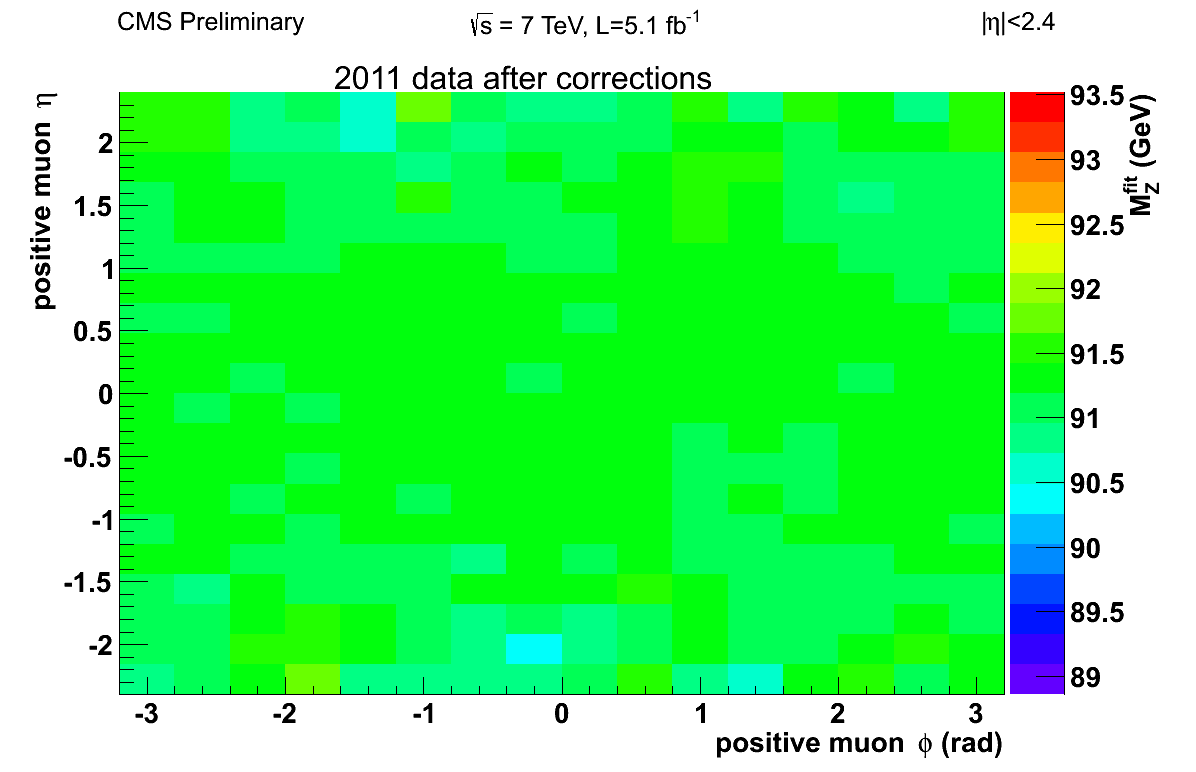
\includegraphics[width=0.45\textwidth]{figures/TkAl_Style/Data2011_44X/MassVsEtaPhiPlus_file1}
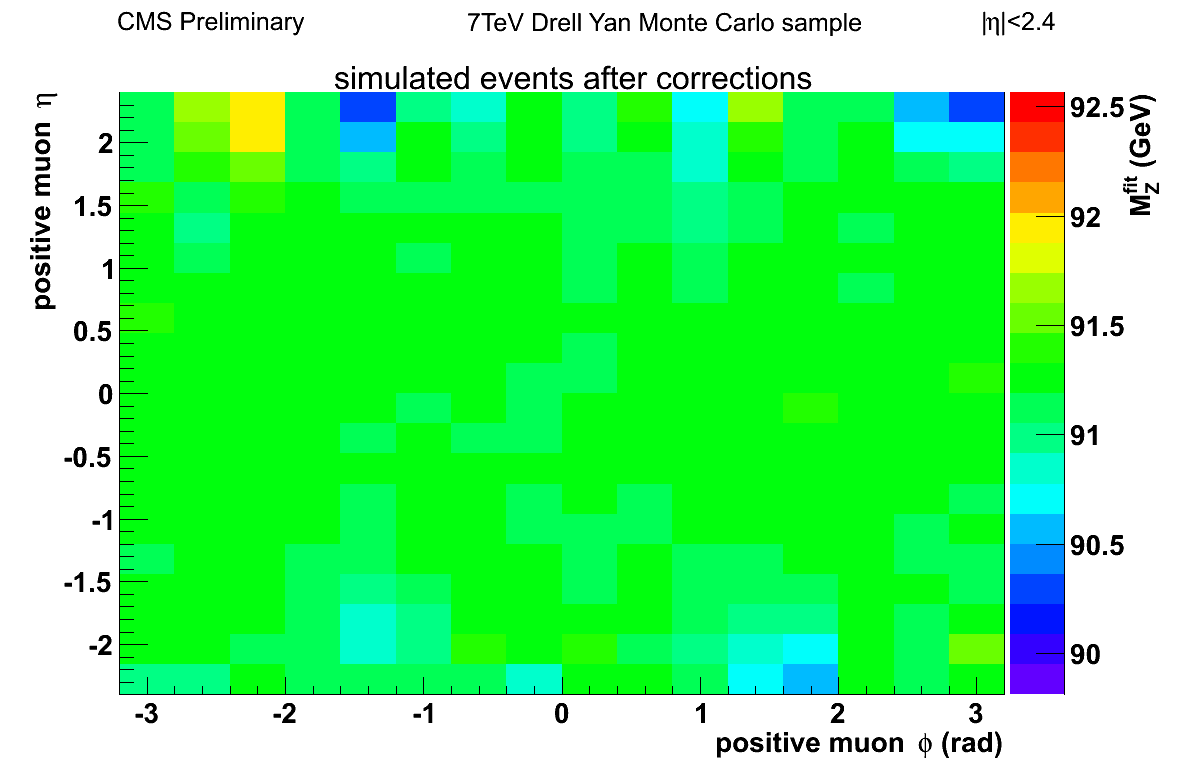
\includegraphics[width=0.45\textwidth]{figures/TkAl_Style/MC2011_44X/MassVsEtaPhiPlus_file1}
 \hspace{1cm} 
   \caption{Mass of the Z extracted from the spectrum of the dimuon
     invariant mass for real (left) and simulated (right) events at $\sqrt{s}$=7 TeV, after
     applying the corrections computed with MuScleFit.
   \label{fig:etaphi_44X_after}}
 \end{center}
\end{figure} 
The beneficial effect of the corrections can be appreciated also
inspecting the resolution of the mass of the Z boson before and after the
corrections. This is shown as a function of the $\eta$ of the positive
muon in Figure~\ref{fig:SigmaVsEta_44X} for real (left) and simulated (right) events 
at $\sqrt{s}$=7~TeV. 
\begin{figure}[hbtp]  
\begin{center}
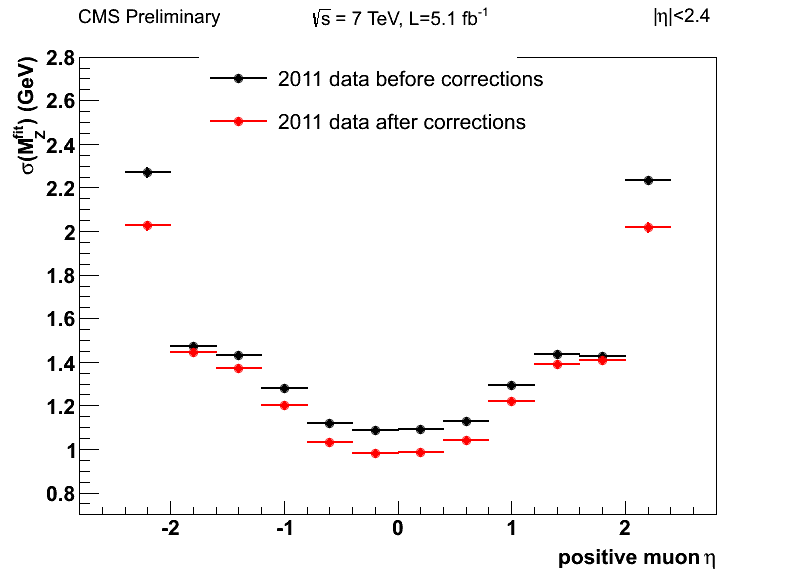
\includegraphics[width=0.45\textwidth]{figures/TkAl_Style/Data2011_44X/SigmaVsEtaPlus}
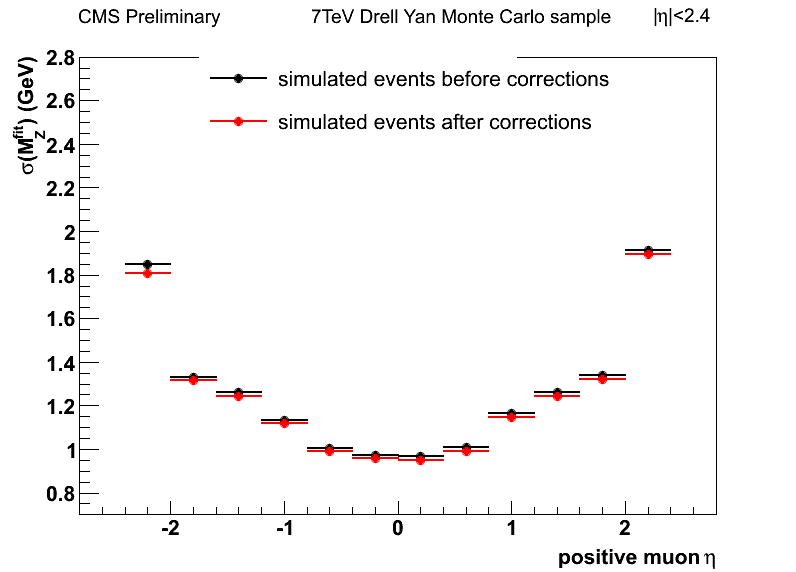
\includegraphics[width=0.45\textwidth]{figures/TkAl_Style/MC2011_44X/SigmaVsEtaPlus}
 \hspace{1cm} 
   \caption{Resolution on the mass of the Z boson extracted from the specturm of the dimuon
     invariant mass for real (left) and simulated (right) events at
     $\sqrt{s}$=7 TeV. Resolutions before and after applying the
     corrections are compared.
   \label{fig:SigmaVsEta_44X}}
 \end{center}
\end{figure} 
Despite the sensible improvement observed in the
data, the resolution in simulated events can be up to 10\%
better. To match the resolution in the simulation with that
measured in the data, a gaussian smearing 
of the curvature of muons was introduced:
\begin{equation}
\kappa' = \kappa + |\kappa| \cdot G(0,s_j).
\label{eq:smearing}
\end{equation} 
$G(0,s_j)$ is a gaussian function with the standard
deviation $s_j$ for the $j^{th}$- $\eta$ bin defined  as:
\[
s_j = \gamma \, \frac{\sqrt{\sigma^2_{data,j}-\sigma^2_{MC,j}}}{p_T}
\] 
with $\sigma_{data,j}$ and $\sigma_{MC,j}$ are the resolutions on
$p_T$ (Eq.~\ref{eq:resolution_function}) in data and simulation and $\gamma$ is a
coefficient, of order unity, empirically determined. 

Figure~\ref{fig:MassRatio_8TeV} shows the ratio of the dimuon spectra
in data and simulation at $\sqrt{s}$=8~TeV, before and after the calibration and smearing
procedure. Background estimated with the exponential function of
Table~\ref{tab:fit_pdfs} were subtracted from the spectra. Overall, after the
correction the position of the peak is matched at the 10$^{-4}$ level
and the resolution at the 10$^{-2}$ level.
\begin{figure}[hbtp]  
\begin{center}
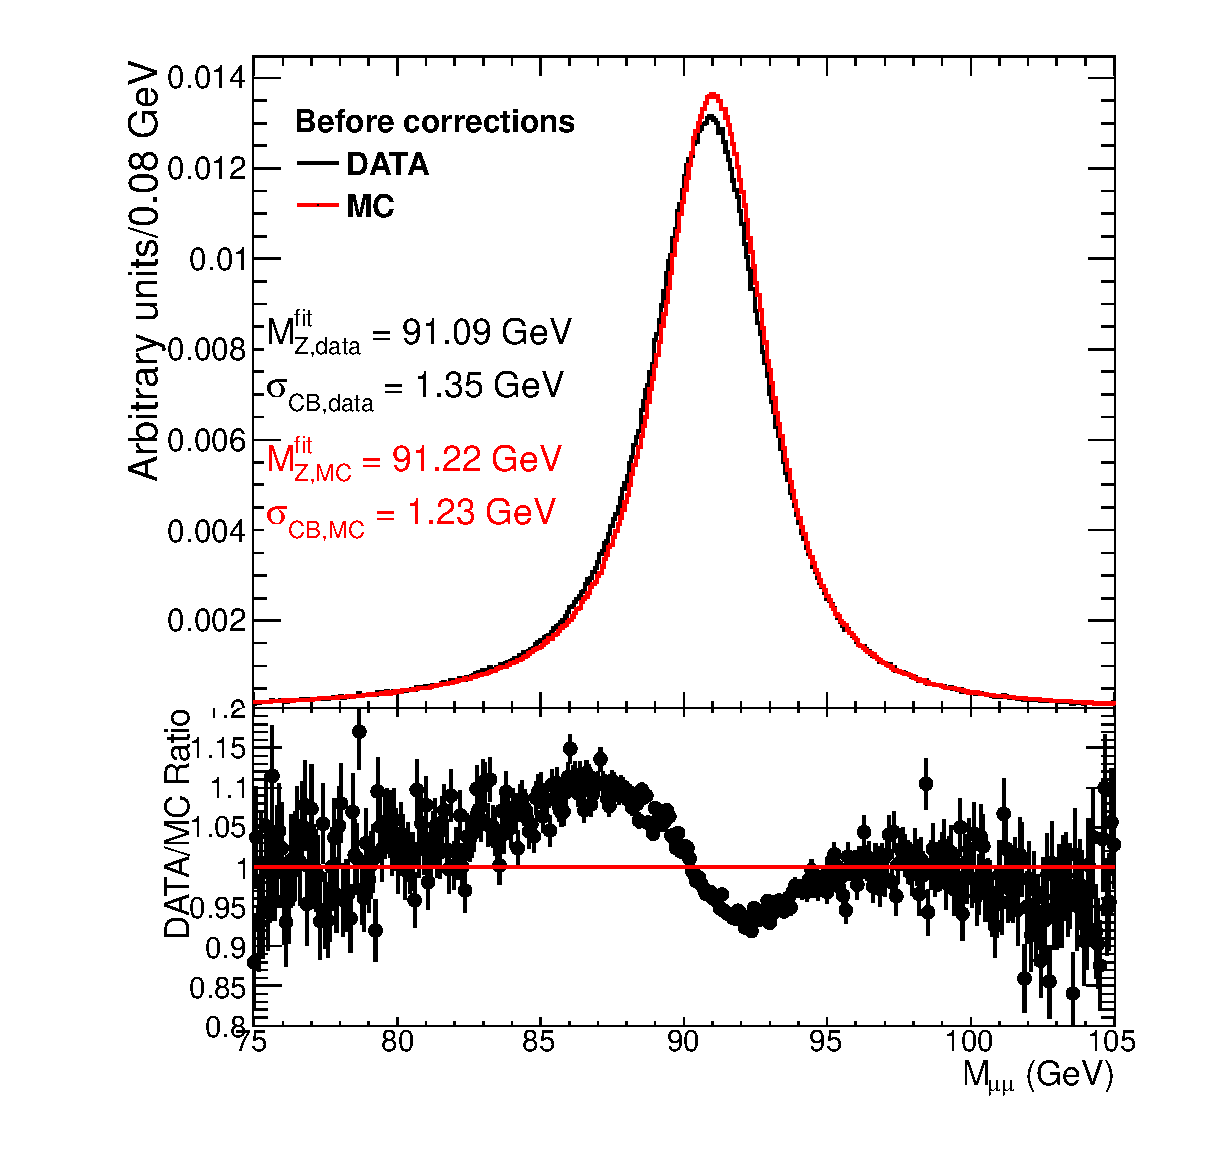
\includegraphics[width=0.7\textwidth]{figures/MassRatio_Style/2012_22Jan2013ReReco/DimuonAfterBkgSub_beforeCorrections} 
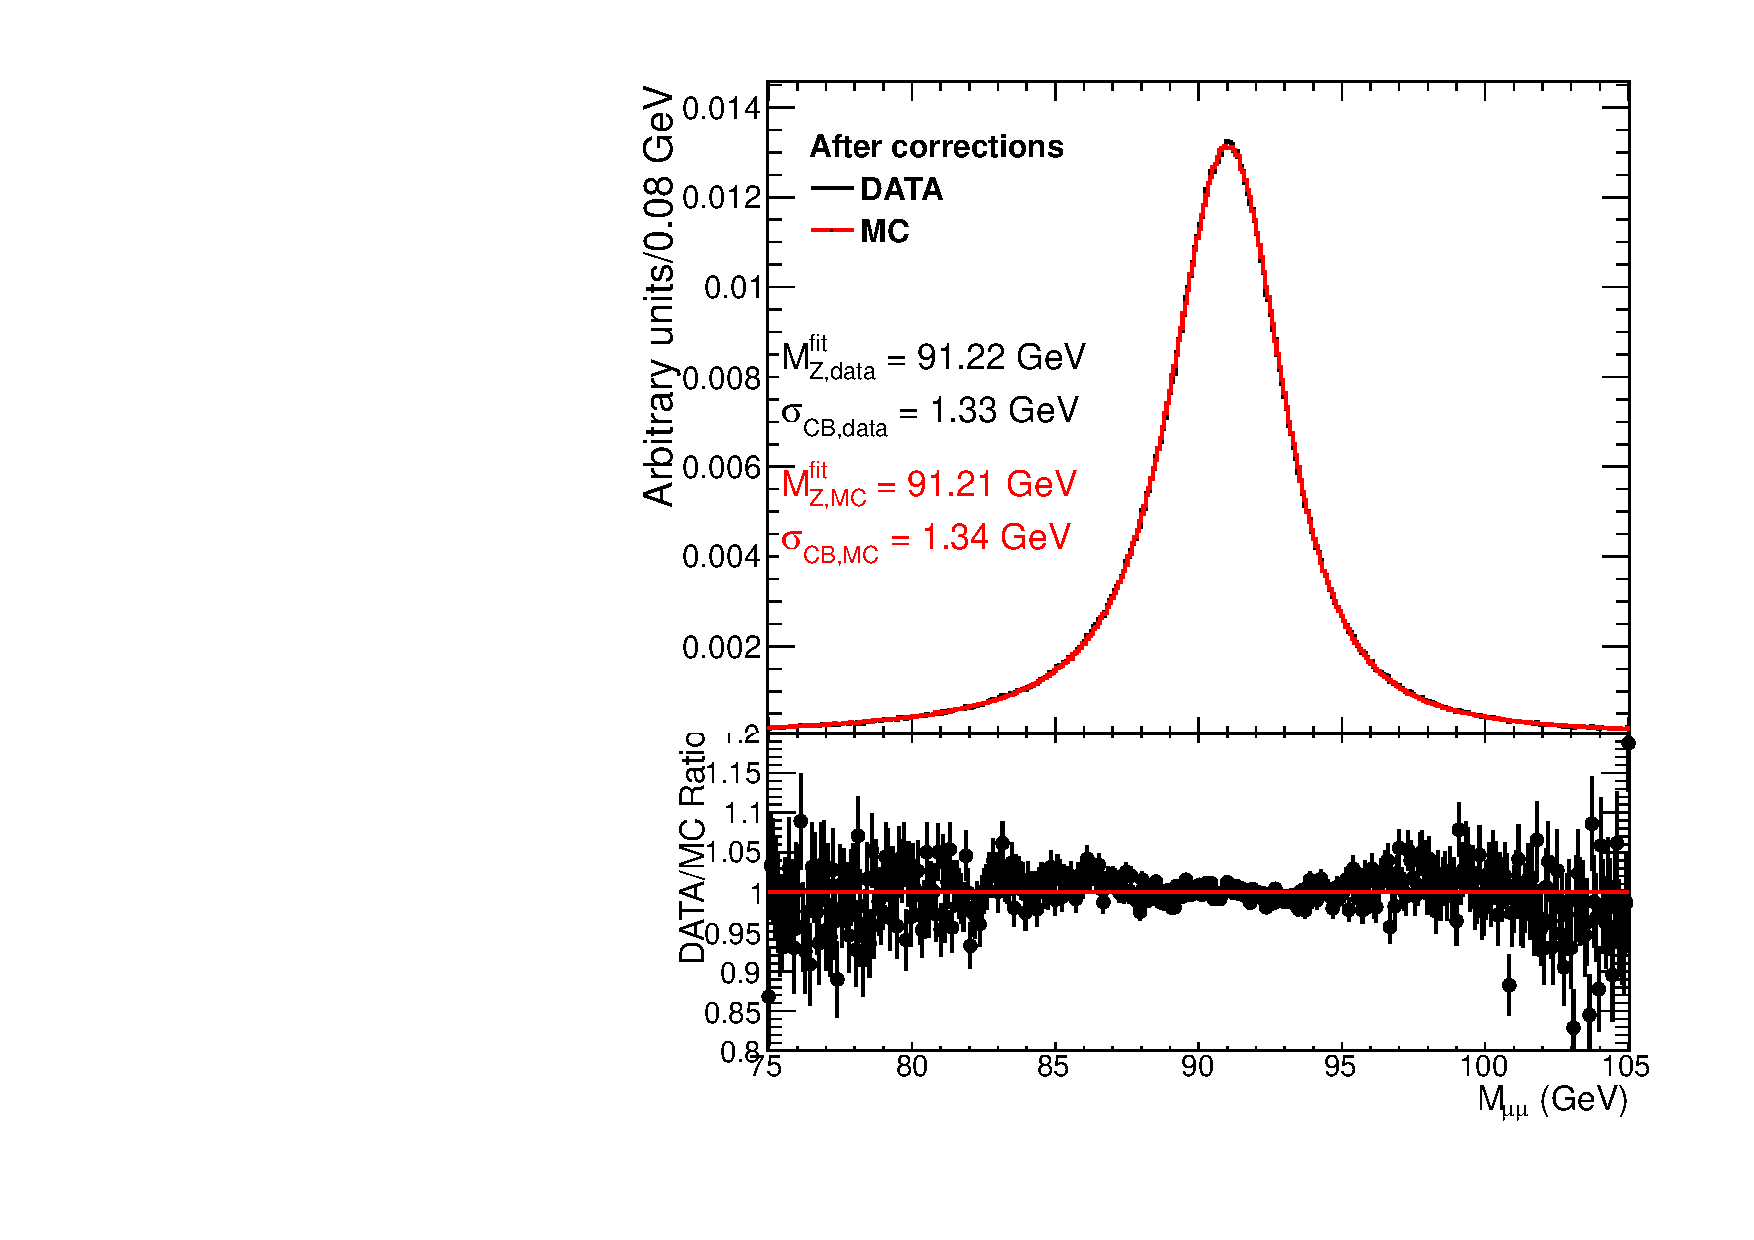
\includegraphics[width=0.7\textwidth]{figures/MassRatio_Style/2012_22Jan2013ReReco/DimuonAfterBkgSub_afterCorrections}
 \hspace{1cm} 
   \caption{Ratio of the backgroud subtracted dimuon
     invariant mass distributions in data and in simulation: before (top) and after
     (bottom) applying the scale correction and smearing.
     Spectra are parametrized with the pdf described in Table~\ref{tab:fit_pdfs}.
   \label{fig:MassRatio_8TeV}}
 \end{center}
\end{figure} 



%%%%%%%%%%%%%%%%%%%%%%%%%%%%%%%%%%
\section{Validation of the results}
%%%%%%%%%%%%%%%%%%%%%%%%%%%%%%%%%%
\begin{itemize}
\item data-driven validation of 2012 corrections
\item datasets
\item definition of eta, pT bins for the different resonances
\item description of the functions used for the fits
\item smearing of the resolution in the simulation
\item results
\end{itemize}
The corrections computed with MuScleFit were validated by comparing the
poistion of pole and the resolution extracted from the spectra of dimuons from
three reference resonances: J/$\psi$, $\Upsilon(1S)$ and Z. 
The models used to fit the resonances are detailed in Table~\ref{tab:fit_pdfs}.
%%%%%%%
\begin{table}[hbH]
\begin{center}
\caption{PDFs \FIXME describe what is $x$, $CB$ and $BW$ \label{tab:fit_pdfs}} 
\begin{tabular}{|ll|c|c|c|}
\hline
Resonance & & Fit Range [GeV] & Signal pdf & Background pdf \\
\hline
J/$\psi$       & DATA & [2.9,3.3] & $CB(x,\mu,\sigma)$ & 3$^{rd}$ order Bern. pol. \\
               & MC   & [2.9,3.3] & $CB(x,\mu,\sigma)$ & 3$^{rd}$ order Bern. pol. \\
\hline
$\Upsilon(1S)$ & DATA & [8.7,11.0] & $CB_(x,\mu_1,\sigma)+CB(x,\mu_2,\sigma)+CB(x,\mu_3,\sigma)$ & 4$^{th}$ order Bern. pol. \\
               & MC   & [8.8,10.0] & $CB_(x,\mu,\sigma)$            & 4$^{th}$ order Bern. pol. \\
\hline
Z              & DATA & [75,105] & $BW \otimes CB$ & $\exp(a_0+a_1x+a_2x^2)$  \\
               & MC   & [75,105] & $BW \otimes CB$ & $\exp(a_0+a_1x+a_2x^2)$  \\
\hline
\end{tabular}
\end{center}
\end{table}

%%%%%%%%%%%%%%%%%%%%%%%%%%%%%%%%%%%%%%%%%%%%%
\section{Study of the systematic uncertainties}
\label{sec:systematics}
%%%%%%%%%%%%%%%%%%%%%%%%%%%%%%%%%%%%%%%%%%%%%
%We estimate the systematic uncertainty on the post-corrections muon momentum 
%as the linear sum of two contributions accounting for the two common use cases:
The validation procedure described in the previous section is used for
estimating the systematic error on the post-correction momentum of the muons.

There are two common use cases for defining a systematic
error on the momentum scale: 
\begin{itemize}
\item {\sl Case I}: analyses where the spectrum in the data is compared
  with a model known from the simulation. Here the systematic error is
  indicated by the residual
  discrepancy between the post-correction
  spectrum in the data and in the simulation.
\item {\sl Case II}: analyses aiming to perform an absolute measurement of the
  momentum of the muon, e.g. not relying on a model for the
  expected spectrum. In this case, values of observables built from the measured
  momenta, namely invariant masses, differing from standard
  references are indications of systematic errors. 
\end{itemize}

\underline{\sl Case I}: We define the systematic error  $\Delta p_T$ related to the remaining discrepancy between
the data and the simulation as:
\begin{equation}
  \frac{\Delta p_T}{p_T}=\frac{M_{DATA}-M_{MC}}{M_{PDG}}
  \label{eq:syst_DATA_MC}
\end{equation}
The above relation between momentum
and masses holds under the hypothesis that the systematic errors are fully correlated between the two muons. 
The fractional difference on the mass is shown as a function of $|\eta|$ or $p_T$ of one of the two muons in
Figure~\ref{fig:ScaleDATAMC_8TeV}.
%%~\ref{fig:syst_DATA_MC_eta}. 
%% \begin{figure}[hbtp]  
%% \begin{center}
%% 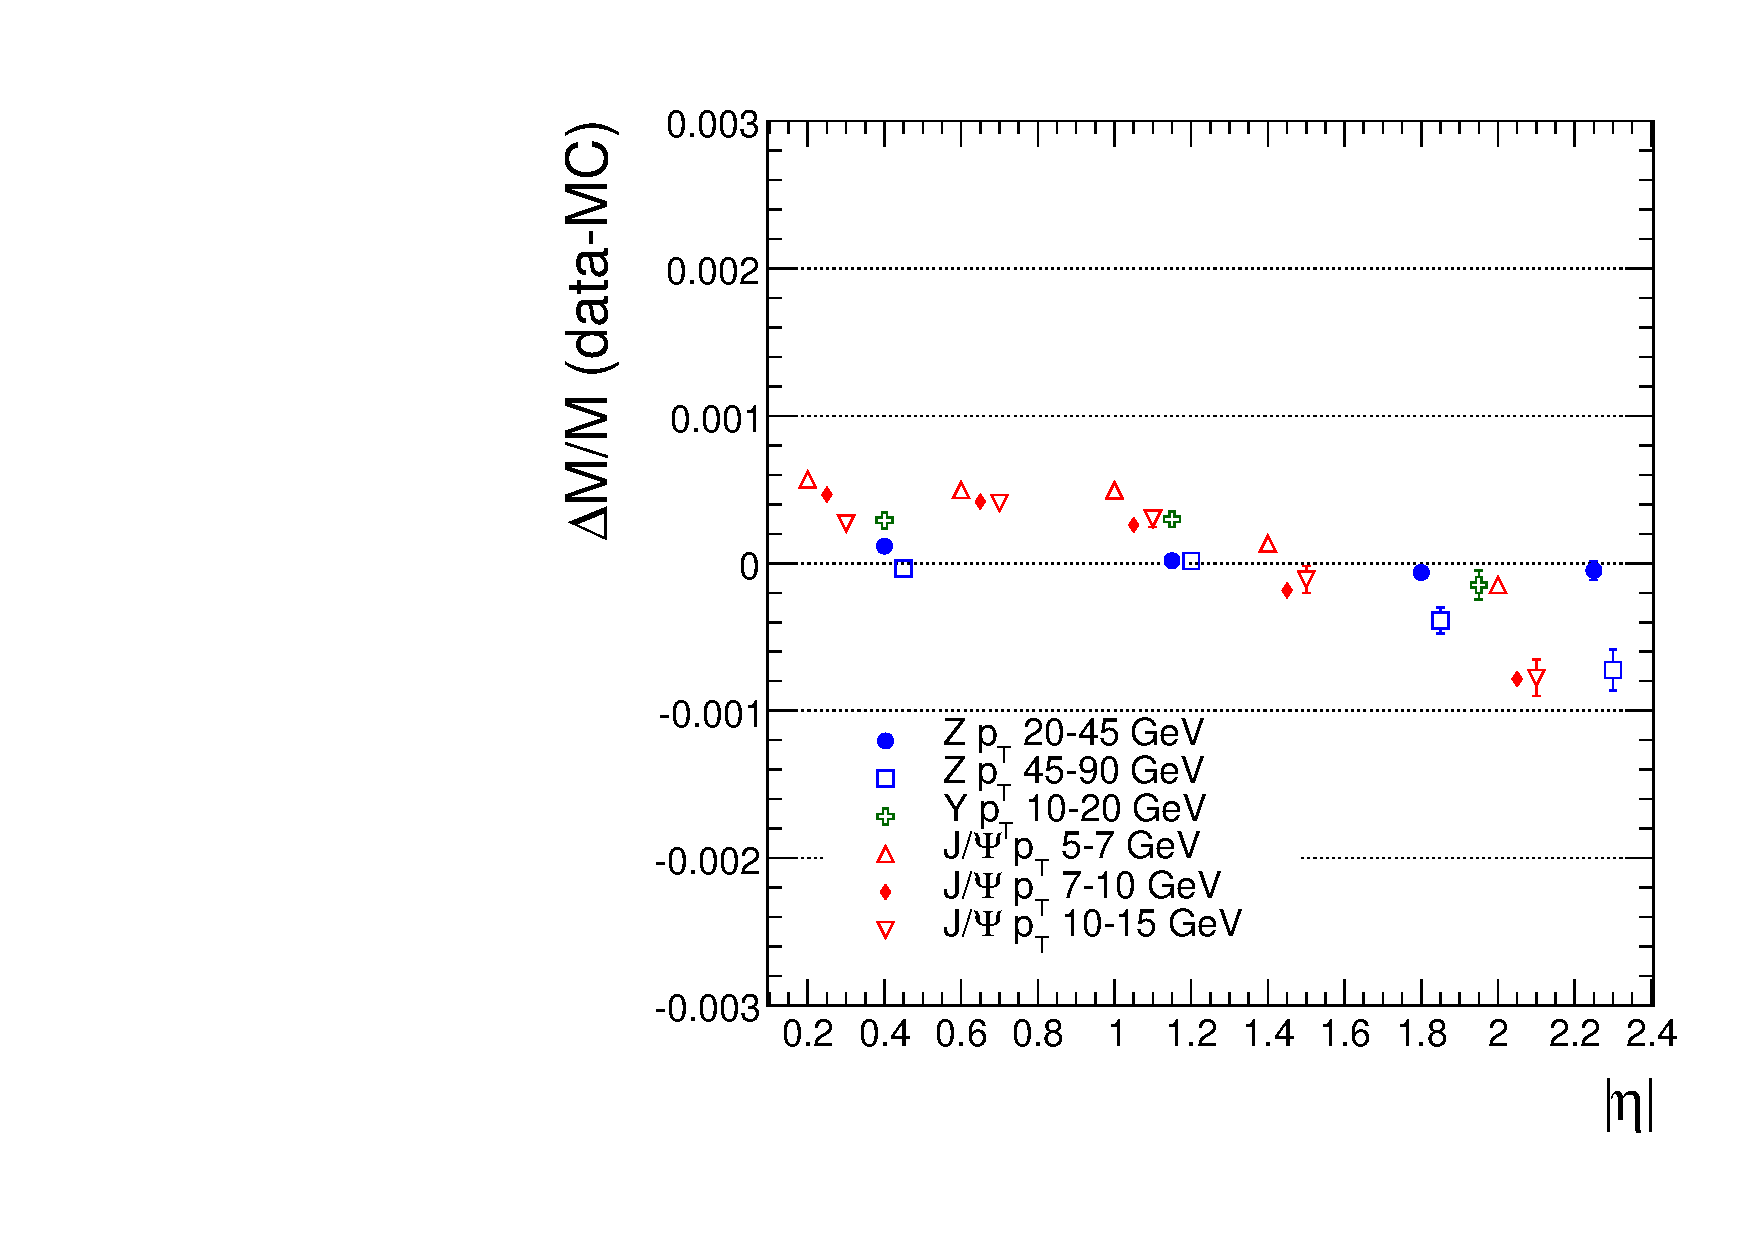
\includegraphics[width=\textwidth]{figures/ScaleEta_afterCorrection_V2}
%%  \hspace{1cm} 
%%    \caption{Fractional difference $\frac{M_{DATA}-M_{MC}}{M_{DATA}}$
%%      for dimuons from J/$\psi$, $\Upsilon(1S)$ and Z decays as a function of the $|\eta|$
%%      of one the two muons (averaged on the second).} 
%%    \label{fig:syst_DATA_MC_eta} 
%%  \end{center}
%% \end{figure} 
The fractional difference is everywhere well within $\pm$0.10\% with the largest value
being around -0.10\%, for the point in the large $|\eta|$ and $p_T$ bin.
Conservatively we assign a $\pm$0.05\% uncertainty everywhere apart from this
point where a $\pm$0.10\% uncertainty is assumed. 

\underline{\sl Case II}: With respect the previuos case, the
systematic error on $p_T$ has an additional contribution that we
evaluate using the simulation and taking as estimator the discrepancy
between the values of the mass of the Z boson extracted from the
spectra of the dimuons and the world average reported by the Particle
Data Group (PDG)~\cite{Beringer:1900zz}: 
\begin{equation}
  \frac{\Delta p_T}{p_T}=\frac{M_{MC}-M_{PDG}}{M_{PDG}}
  \label{eq:syst_MC_PDG}
\end{equation}
The above relation between momentum
and masses holds under the hypothesis that the systematic errors are fully correlated between the two muons. 
%Ideally after the calibration procedure, both in
%the simulation and in the data, 
We checked the behaviour of the fractional mass difference defined
in Eq.~\ref{eq:syst_MC_PDG} against $p_T$ and $|\eta|$ of one of the two
muons using simulated events reconstructed in realistic conditions
(Figure~\ref{fig:ScalePDGMC_8TeV}). 
%%%%
\begin{figure}[hbtp]  
\begin{center}
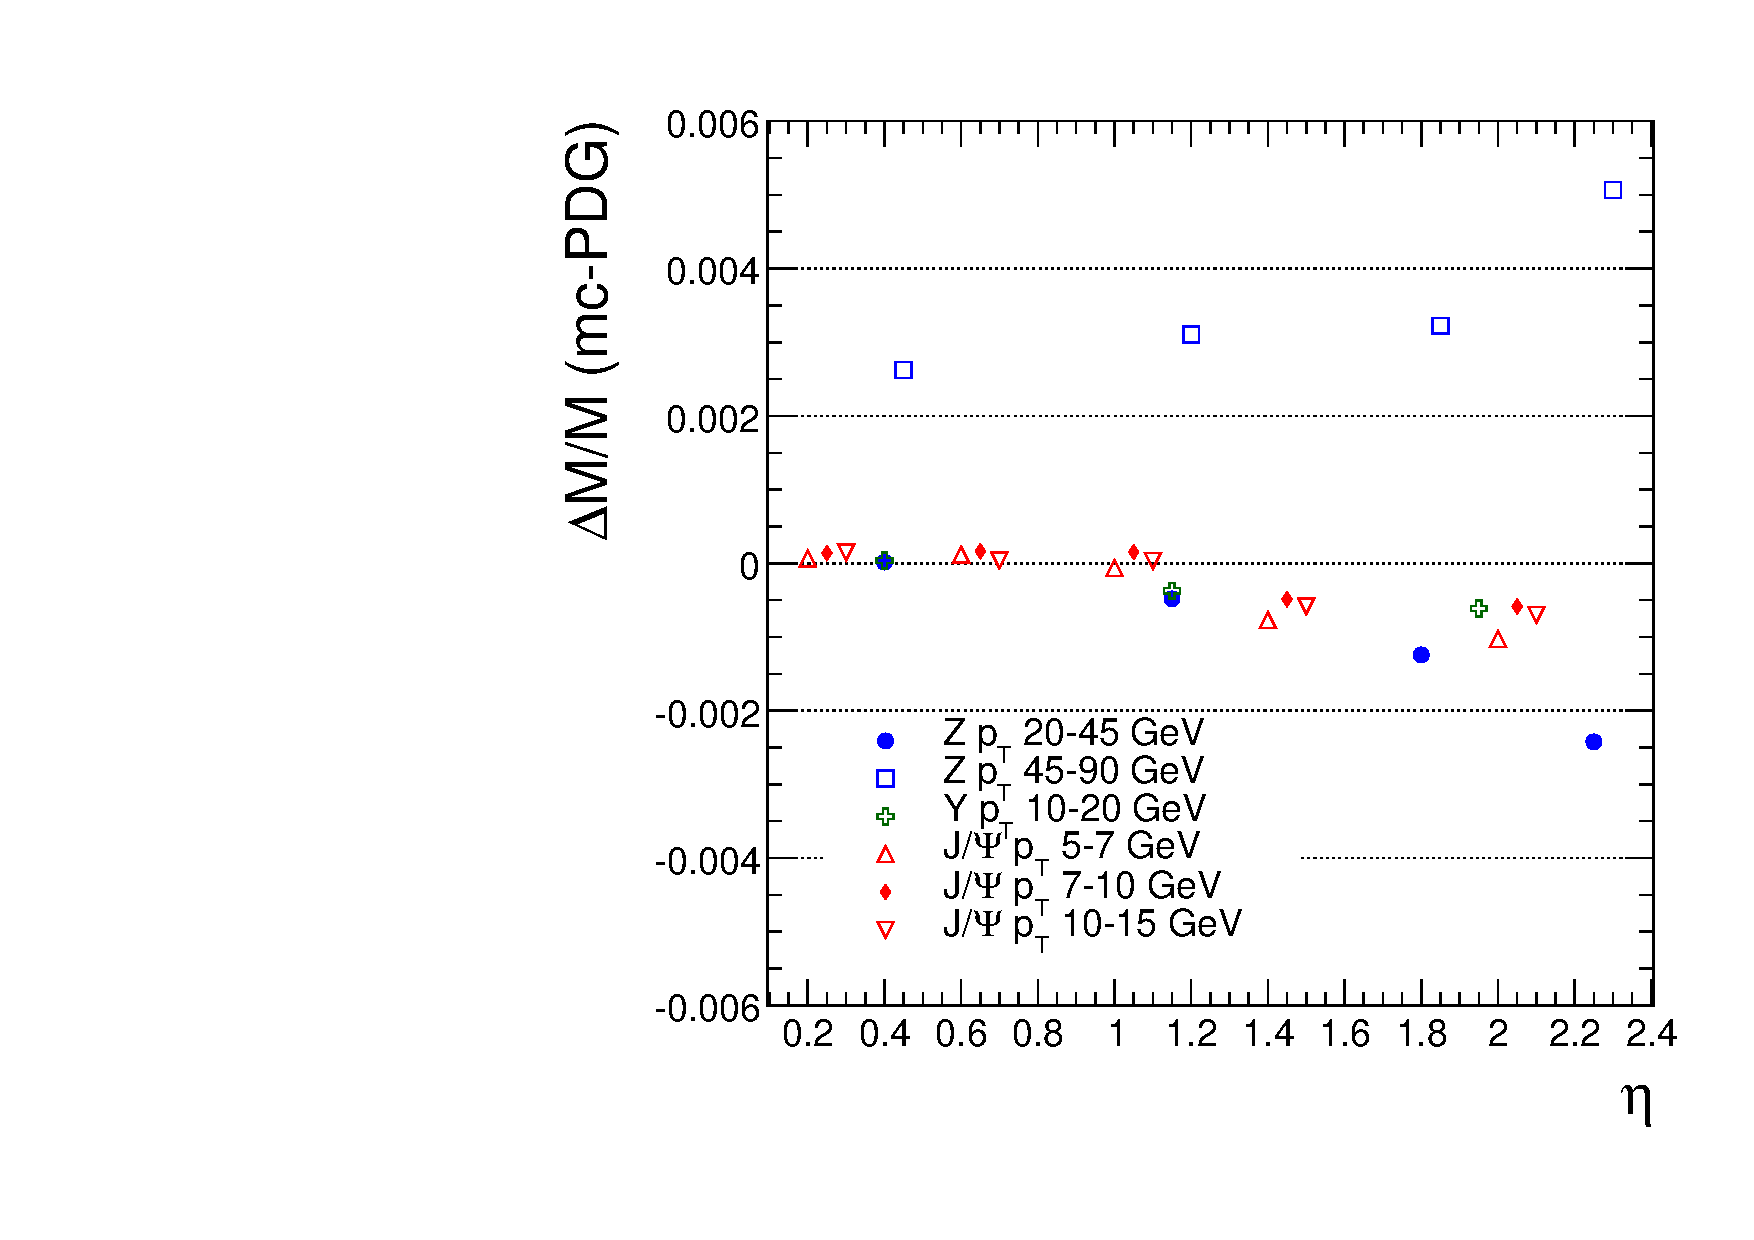
\includegraphics[width=0.7\textwidth]{figures/H4l_Style/2012_22Jan2013ReReco/ScalePdg_mc_Eta_afterCorrection_V2}
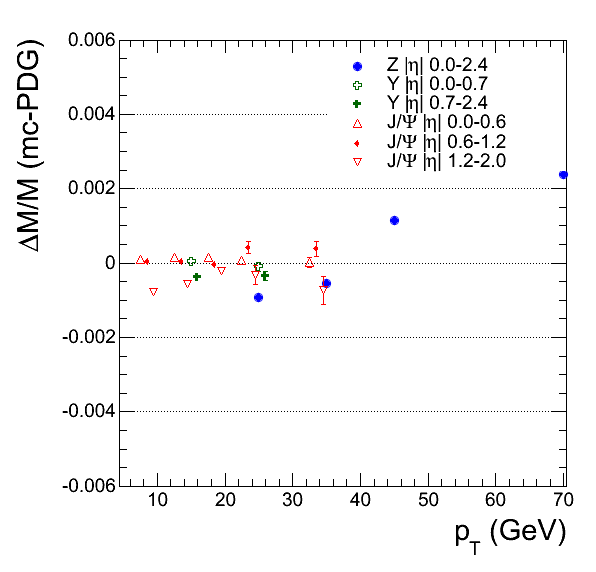
\includegraphics[width=0.7\textwidth]{figures/H4l_Style/2012_22Jan2013ReReco/ScalePdg_mc_Pt_afterCorrection_V2} 
 \hspace{1cm} 
   \caption{Fractional difference, PDG with respect simulation, of the fitted mass for the J/$\psi$,
     $\Upsilon(1S)$ and Z resonances as a function of the $|\eta|$ (top)
     and $p_T$ (bottom) of one of the two muons. Bars are the
     statistical error on the mass of the resonance from the fit.
   \label{fig:ScalePDGMC_8TeV}}
 \end{center}
\end{figure} 
Discrepancies from the PDG values, especially visible in the case of
the dimuons from Z, arise either
from a poor parametrization of the dimuon spectrum used to extract $M_{MC}$ or from biases on the muon momentum not entirely corrected by the
calibration procedure.
% %%%
% realistic conditions -> 
% which should reflect the
% level of knowledge of the calibration and alignment conditions which
% reflects their accuracy in the data. 
% %%%  TO BE DEFINED IN EARLIER  SECTIONS 
Since a not null value contributes 
to the {\sl Case II} error,
we disentangled the two effects using
simulated events reconstructed using the so-called {\sl ideal}
conditions , e.g. assuming a perfect knowledge of the
calibration and alignment conditions but with the same set of
dead channels as in real data.
In this sample, biases in the measured momentum due
to approximations in the track reconstruction (e.g. mismodelling
of the interaction of the charged particle
with the material or with the magnetic field during the reconstruction step) were the same as
in the reference sample reconstructed with realistic conditions. 
No MuScleFit corrections were applied to the muons reconstructed with ideal conditions.
Details on the samples used for this test are given in Table~\ref{tab:datasets_for_systematics}.
%%%%%%%
\begin{table}[hbH]
\begin{center}
\caption{Datasets \label{tab:datasets_for_systematics}} 
\begin{tabular}{|l|c|c|c|c|}
\hline
Dataset & MC generator & Data-Tier & events & Corrections applied\\
\hline 
DYJetsToLL & MadGraph &  AODSIM              & 2.95 M & MuScleFit \\
DYToMuMu   & POWHEG   &  AODSIM              & 8.60 M & MuScleFit \\
DYToMuMu   & POWHEG   &  START\_53 from RECO & 0.59 M & MuScleFit \\
DYToMuMu   & POWHEG   &  MC\_53 from RECO    & 0.59 M & nocorrections \\
\hline
\hline
\end{tabular}
\end{center}
\end{table}
%%%%
\begin{figure}[hbtp]  
\begin{center}
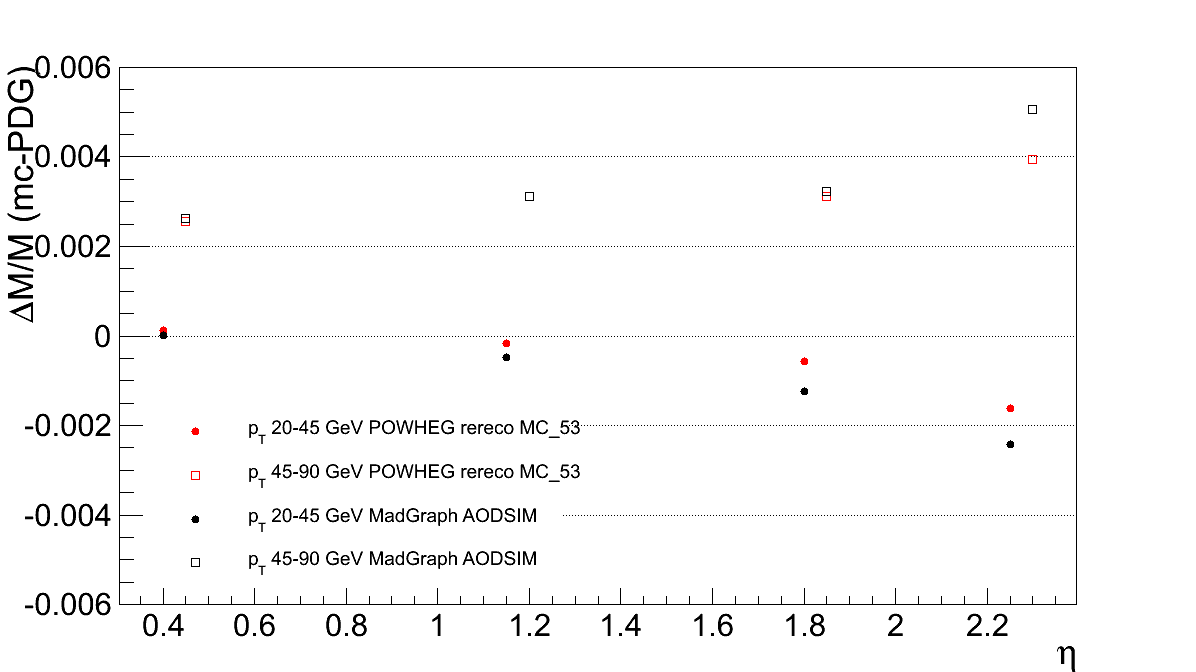
\includegraphics[width=\textwidth]{figures/ScalePdg_mc_Eta_Z}
 \hspace{1cm} 
   \caption{Fractional difference, PDG with respect simulation,
     for dimuons from Z bosons decays as a function of the $|\eta|$
   of one the two muons (averaged on the second).} 
   \label{fig:syst_MC_PDG_eta} 
 \end{center}
\end{figure} 
%Figure~\ref{fig:syst_MC_PDG_pT} shows the fractional difference on the
%mass as a function of $p_T$ of one of the
%two muons. Points for realistic simulation (post-correction) show a
%bias increasing with $p_T$. The same trend is observed for the points
%obtained with the ideal simulation which agree the with the others 
%at the 0.0005 level on all the $p_T$ range. 

Figure~\ref{fig:syst_MC_PDG_eta} shows the fractional difference on
the mass as a function of $|\eta|$ of one of the two muons in two
different ranges of $p_T$ for the ideal and the realistic samples:
\begin{itemize}
\item for $p_T$ in the range [20,45] GeV, values
form the realistic simulation (post-correction) are off of about -0.05\%
for $|\eta|<$1.5 increasing up to -0.20\% at the largest $|\eta|$.
A similar trend, but with smaller offsets, is observed for points from the simulation in ideal
conditions. 
\item for $p_T$ in the range [45,90] GeV there is approximately
a +0.20\% bias growing up to +0.50\% at the largest $|\eta|$ bin
in case of both ideal and realistic conditions. 
\end{itemize}
For the muons in the sample reconstructed with ideal conditions, 
we found that the bias in the mass was similar to what determined
comparing the reconstructed $p_T$ with the value from the
MC-truth. This test indicates the overall reliablility of the fits
to the dimuon spectra. Consequently we used the fractional differences
defined by Eq.~\ref{eq:syst_MC_PDG} to estimate the difference between 
true and reconstructed $p_T$ in the realistic simulation.

Based on this analysis, the systematic errors on the momentum scale of
muons in the data, estimated for the
different $p_T$ and $|\eta|$ ranges are those summarized in
Table~\ref{tab:systematics}. {\sl Case II} systematic errors are the sum of the
second and third columns in the table.
%%%%%%%
\begin{table}[hbH]
\begin{center}
\caption{Estimated systematic uncertainties on the momentum scale
  of muons, post-correction, reconstructed in the data ($\Delta p_T/p_T$).
  Second column corresponds to {\sl Case I} systematics, while
  the sum of second and third columns corresponds to {\sl Case II}
  systematics described in the text.\label{tab:systematics}} 
\begin{tabular}{|l|c|c|}
\hline
 & DATA - MC & MC - PDG \\
\hline 
$p_T<$45 GeV,   0$<|\eta|<$1.5 & $\pm$0.05\%& $\pm$0.05\% \\
$p_T<$45 GeV, 1.5$<|\eta|<$2.4 & $\pm$0.10\%& $\pm$0.20\% \\
$p_T>$45 GeV,   0$<|\eta|<$2.0 & $\pm$0.05\%& $\pm$0.30\% \\
$p_T>$45 GeV, 2.0$<|\eta|<$2.4 & $\pm$0.10\%& $\pm$0.50\% \\
\hline
\hline
\end{tabular}
\end{center}
\end{table}
%%%%

%% **DO NOT REMOVE BIBLIOGRAPHY**
\bibliography{auto_generated}   % will be created by the tdr script.

%%% DO NOT ADD \end{document}!

